\documentclass[10pt,a4paper,notitlepage]{report}
\usepackage[utf8]{inputenc}
\usepackage{amsmath}
\usepackage{amsfonts}
\usepackage{amssymb}
\usepackage{hyperref}
\usepackage[margin=1in]{geometry}
\usepackage{fancyhdr}
\usepackage[svgnames]{xcolor}
\usepackage{graphicx}
\usepackage{minted}

\usemintedstyle{manni}
\pagestyle{fancy}
\fancyhead[L]{\small Decoding Neuronal EEG Activity}
\fancyhead[R]{\small\textsc{Problem 1}}
\renewcommand{\headrulewidth}{0.4pt}
\fancyfoot[C]{\thepage}

%\newcommand{\code}[1]{\colorbox{lightgray}{\texttt{#1}}}

\begin{document}

\paragraph*{GENERAL REMARKS} The programming problems require you to fill the gaps in the provided MATLAB scripts. Use the problem description below and the comments in the code to solve the problems. The missing parts are typically indicated by '\texttt{...}' (not to be confused with line breaks!), where each '\texttt{...}' might be replaced by multiple lines of code. Following the provided code is recommended but only leads you to one of many possible solutions. If some part of the code seems unclear or counterintuitive to you, feel free to depart from it. Be aware, however, that the suggested variable names and structures are typically used later in the script, e.g. for plotting, and occur again in other scripts and problems. In any case, your code should produce the same output as the Musterlösung. \textbf{Note}: To be able to run the code, you must have the Statistics, Signal Processing, Image Processing, and Wavelet toolboxes installed, and you must have the folder \texttt{utility} and all subfolders as well as the location of the ECG/EEG datasets added to your MATLAB path.

\section*{Problem 1}
In this problem, we will generate bivariate data from two normal distributions and classify the data using logistic regression. \texttt{runTest.m} executes the main part of the program and calls \texttt{modelFitVal.m} to fit and cross-validate the model. We will visualize the underlying distributions and the resulting decision boundary.

\section*{Part 1: Sampling and Analyzing}
\texttt{runTest.m} begins by specifying the parameters for generating the data: sample size, means, and covariance matrix.

\begin{minted}[xleftmargin=1cm]{matlab}
nSamples = 500;
mu1 = [1,3];
mu2 = [3,0];
sigma = [2.0 1.5
         1.5 2.0];
\end{minted}

First, we generate the data using these parameters and an appropriate function, concatenate the two sample populations, and create a vector of labels (ones for one population, zeros for the other).

\begin{minted}[xleftmargin=1cm]{matlab}
X1 = ...
X2 = ...
X = [X1; X2];
L = ...
\end{minted}

\texttt{X} will be a 2*\texttt{nSamples}$\times$2 matrix and \texttt{L} will be of length 2*\texttt{nSamples}.

Next, we want to see what the two underlying distributions look like along the two dimensions $x_1$ and $x_2$ (not to be confused with the two sample populations \texttt{X1} and \texttt{X2}). Create a grid of 100$\times$100 equidistant points within the bounds of the sample populations, using \texttt{xVector}, and compute the two PDFs for each point.

\begin{minted}[xleftmargin=1cm]{matlab}
xVector = linspace(min(X(:)), max(X(:)), 100);
...
pX1 = ...
pX2 = ...
pDist = reshape(pX1 + pX2, 100, 100);
\end{minted}

You might want to use the \texttt{meshgrid} function and reshape the resulting matrices to vectors. If you have trouble with the suggested one-liners, use for-loops instead. The result \texttt{pDist} should be a 100$\times$100 matrix containing the sum of both PDFs.

Now we train a generalized linear model on the sample data to perform logistic regression. Look into the MATLAB documentation for \texttt{glmfit} to find the right arguments for the distribution and link function.

\begin{minted}[xleftmargin=1cm]{matlab}
coeff = glmfit(...);
\end{minted}

The result \texttt{coeff} will be a vector of 3 coefficients.

To display the decision boundary of the fitted model, we solve the iso-error problem, i.e. we compute the line on which $P(C_1|x) = P(C_2|x) = 0.5$. This means solving
\begin{equation*}
0.5 = \sigma (w^Tx+w_0)
\end{equation*}
with $\sigma$ being the logistic function; $w=(w_1,w_2)$; $w_0$, $w_1$ and $w_2$ given by \texttt{coeff}; and $x=(x_1,x_2)$. We have to rewrite the equation for $x_2$ and set $x_1$ to \texttt{xVector}.

\begin{minted}[xleftmargin=1cm]{matlab}
x2db = ...
\end{minted}

Now we validate the fitted model (find the appropriate function!) on the same 100$\times$100 data points as before to get the posterior densities predicted by the model. (We only compute $P(C_1|x)$, since $P(C_2|x)=1-P(C_1|x)$.)

\begin{minted}[xleftmargin=1cm]{matlab}
posteriorC1 = ...
posteriorC1 = reshape(posteriorC1, 100, 100);
\end{minted}

Finally, we want to again train and 10-fold cross-validate the model, using our own function.

\begin{minted}[xleftmargin=1cm]{matlab}
kCross = 10;
pCorrect = modelFitVal(X, L, kCross);
\end{minted}

The remainder of \texttt{runTest.m} is about plotting and doesn't need to be edited.

\section*{Part 2: Classification}
The function \texttt{modelFitVal.m} should take a data matrix (samples$\times$dimensions), a correpsonding label vector, and the number of partitions, then iteratively divide the data and labels into training sets and test sets, fit and validate the GLM, and return the mean percentage of correctly predicted labels.

First, we create a random permutation of the sample indices, which we will use when composing the partitions.

\begin{minted}[xleftmargin=1cm]{matlab}
nSamples = size(X, 1);
randIdx = ...
\end{minted}

This way we avoid order effects on model performance but still create disjoint partitions. With our random data, order doesn't matter, but will in the later problems.

In the subsequent loop we divide the data and labels into test and training sets. From \texttt{randIdx} we select $\frac{\texttt{nSamples}}{\texttt{k}}$ indices for testing and the remaining $\frac{(\texttt{k}-1)\texttt{nSamples}}{\texttt{k}}$ indices for training.

\begin{minted}[xleftmargin=1cm]{matlab}
pCorrect = 0;
for iPart=1:k
    idxTest = ...
    idxTrain = ...
    xTest = X(...);
    xTrain = X(...);
    lTest = L(...);
    lTrain = L(...);
\end{minted}

Note that \texttt{nSamples} need not be a multiple of \texttt{k}. Make sure that the size of test sets (same for training sets) does not differ by more than 1 across partitions. Make also sure that all samples are used for testing exactly once.

Now we fit the logit model as before and compare the rounded validation output, i.e. the predicted labels for the test data, to the actual labels. The percentage of correct predictions is then accumulated over iterations.

\begin{minted}[xleftmargin=1cm]{matlab}
    coeff = glmfit(...);
    lPredicted = round(...);
    pCorrect = pCorrect + 1/k*mean(lPredicted==lTest);
end
\end{minted}

\section*{Part 3: Plotting and Exploring}
Your code should print the model's average classification performance and produce the two figures below, showing the sample data with their underlying distributions and the model's decision boundary, and the class posterior probabilities, respectively.

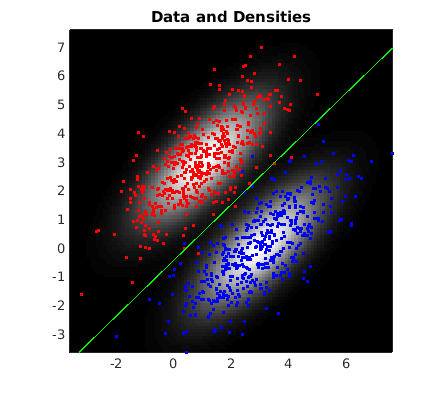
\includegraphics[scale=0.6]{p1fig1.png}
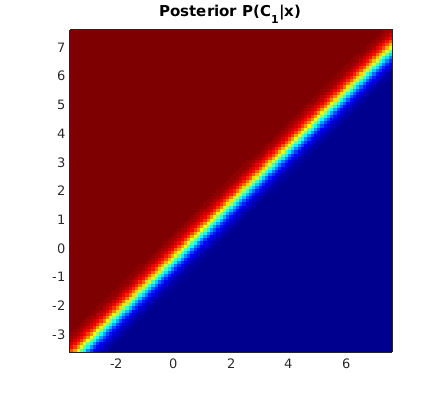
\includegraphics[scale=0.6]{p1fig2.png}

Note that the plots will vary a bit at between runs because of the randomness in sampling and cross-validation. Classification performance should be at or near 100 \%. You may want to try different distribution parameters and sample sizes and see how performance and plots change. Try to understand the warning messages you might get.

\end{document}
